\section{Alternativas Neurossimbólicas} % Seções são adicionadas para organizar sua apresentação em blocos discretos, todas as seções e subseções são automaticamente exibidas no índice como uma visão geral da apresentação, mas NÃO são exibidas como slides separados.

\begin{frame}
	\frametitle{OG-RAG}
	{\footnotesize
		\begin{itemize}
			\item O OG-RAG é uma arquitetura que adiciona uma \textbf{ontologia curada por humanos} ao processo de \textit{chunking} dos documentos de domínio  representado nos documentos
			\item Uma \textit{ontologia} é uma representação simbólica do conhecimento do domínio representado nos documentos
			\item  A \textbf{ontologia} é curada por especialistas do domínio e permite que cada \textit{chunk} carregue a semântica formal do conhecimento representado nos documentos
		\end{itemize}
	}
	\begin{figure}[H]
		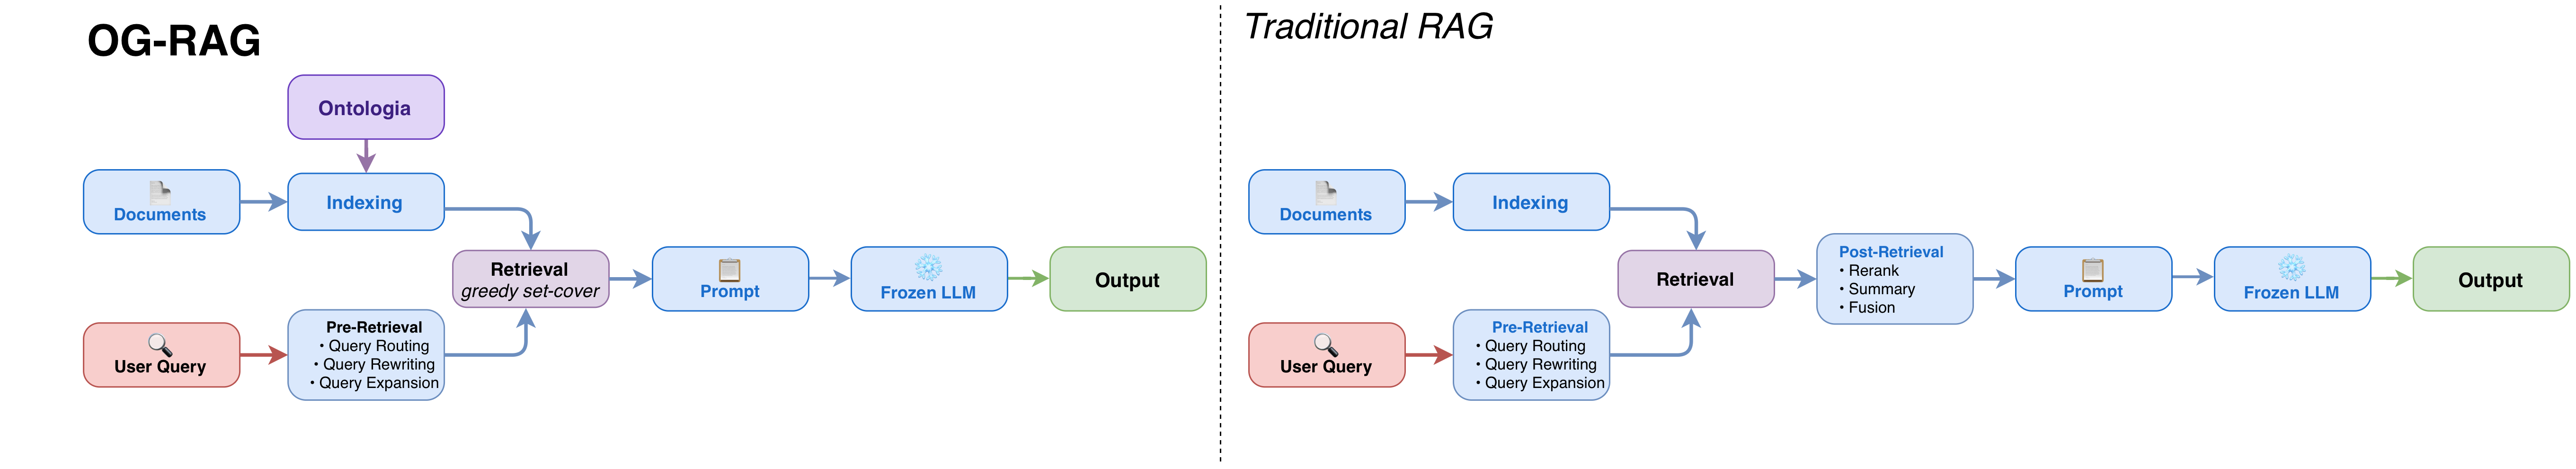
\includegraphics[width=1.0\linewidth]{img/og_rag_vs_trad_rag.png}
	\end{figure}
\end{frame}

\begin{frame}
	\frametitle{GraphRAG}
	{\footnotesize
		\begin{itemize}
			\item O GraphRAG é uma arquitetura que, na indexação, usa um \textbf{LLM} para extrair \textbf{entidades e relações} dos documentos, construindo um \textbf{grafo de conhecimento sintético}
			\item As entidades são agrupadas em \textbf{comunidades}, e o LLM gera um \textit{community report} (resumo) para cada uma
			\item O \textit{retrieval} assume duas formas: \textbf{\textit{Local Search}}, que percorre o grafo a partir das entidades extraídas da \textit{query}, e \textbf{\textit{Global Search}}, que agrega os \textit{community reports} via \textbf{Map-Reduce}
		\end{itemize}
	}
	\begin{figure}[H]
		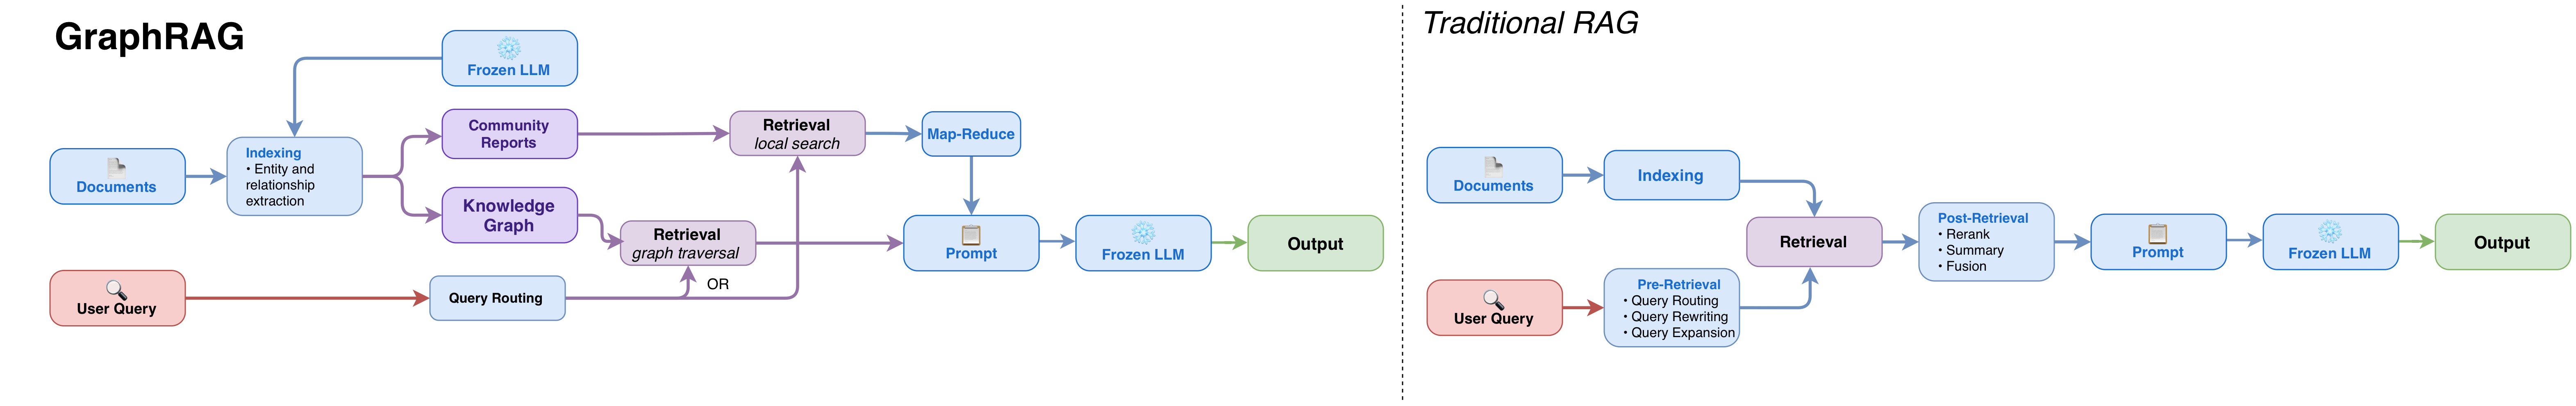
\includegraphics[width=1.0\linewidth]{img/graphrag_vs_trad_rag.png}
	\end{figure}
\end{frame}